\setcounter{secnumdepth}{4}
\lstdefinestyle{csharp}{
    language=C#,
    basicstyle=\ttfamily\small,
    commentstyle=\color{green!40!black},
    keywordstyle=\color{blue},
    numberstyle=\tiny\color{gray},
    numbers=left,
    stepnumber=1,
    numbersep=5pt,
    backgroundcolor=\color{white},
    showspaces=false,
    showstringspaces=false,
    showtabs=false,
    tabsize=2,
    frame=single,
    rulecolor=\color{black},
    captionpos=b,
    breaklines=true,
    breakatwhitespace=false,
    title=\lstname,
    escapeinside={\%*}{*)},
morekeywords={var},
}

\chapter{Feinkonzept und Realisierung}

\section{Entwicklungsumgebungen}
\subsection{Visual Studio 2022}
Visual Studio 2022 ist eine integrierte Entwicklungsumgebung (IDE) von Microsoft, die speziell für die Entwicklung von
Softwareanwendungen, Webanwendungen und Desktop-Anwendungen konzipiert ist. Es handelt sich um eine umfangreiche
Entwicklungsumgebung, die von Entwicklern weltweit für eine breite Palette von Anwendungsfällen eingesetzt wird.

\subsection{Unity Editor}
Der Unity-Editor ist eine leistungsstarke integrierte Entwicklungsumgebung (IDE) und eine zentrale Arbeitsumgebung
für die Erstellung von 2D-, 3D-, Augmented Reality (AR) und Virtual Reality (VR) Anwendungen und Spielen. Er wird von
Unity Technologies entwickelt und ist die Hauptplattform für die Entwicklung von Unity-basierten Projekten.

\section{Objektdesign mittels Blender}
\subsection{Rendering und Optimierung für AR}
Bei der Erstellung von 3D-Modellen für Augmented Reality (AR) ist die Optimierung entscheidend, um eine reibungslose
Erfahrung auf Geräten wie der Hololens 2 zu gewährleisten. In Blender können verschiedene Techniken angewendet werden,
um die Modelle für AR zu optimieren.\\
\\
Eine dieser Techniken ist die Polygonreduktion, bei der die Anzahl der Polygone in den Modellen reduziert wird, um die
Belastung für die Hardware zu verringern. Blender bietet Werkzeuge wie den Decimate Modifier, um die Anzahl der Polygone
effizient zu reduzieren, ohne die visuelle Qualität stark zu beeinträchtigen. Es ist essentiell, von Anfang an eine
Modellierungspraxis mit geringer Polygonanzahl zu berücksichtigen. Ein erfahrener Modellierer kann identische Figuren
mit reduziertem Polygonaufwand im Vergleich zu einem Anfänger erstellen, aufgrund seines fundierten Wissens über die
Modellierung von Formen.\\
\\
Bei der Texturenoptimierung sollte auf die Größe und Qualität der Texturen geachtet werden, da übermäßig große Texturen
die Leistung beeinträchtigen können. Blender ermöglicht die Anpassung von Texturauflösung und -komprimierung. Im Verlauf
der Texturierung wurde die Hololens mehrmals in Verbindung mit den Texturen integriert, um sicherzustellen, dass keine
signifikanten Leistungseinbußen auftreten. Wenn Beeinträchtigungen festgestellt wurden, wurden Anpassungen vorgenommen,
indem die Auflösung oder die Reflexionsstufen modifiziert wurden.\\
\\
Es ist empfehlenswert, verschiedene Detailstufen zu implementieren, insbesondere wenn sich der Betrachter von einem
Modell entfernt. Dies kann erreicht werden, indem verschiedene Modellversionen mit unterschiedlichen Polygonanzahlen
erstellt werden. \textbf{(hab ich nicht gemacht, vielleicht mach ichs aber noch deswegen lass ich das stehen)}

\subsection{Export- und Integrationsprozess}
Die nahtlose Integration von Blender-Modellen in AR-Entwicklungsumgebungen ist entscheidend. Es sollten folgende
Aspekte berücksichtigt werden:\\
\\
\textbf{Dateiformat}\\
Blender unterstützt einige Dateiformate für den Export, aber da wir Unity nutzen, haben wir uns für Filmbox (FBX)
entschieden. Das FBX-Dateiformat (Filmbox) ist ein proprietäres Dateiformat, das von Autodesk entwickelt
wurde. Es dient dem Austausch von 3D-Modellen, Animationen, Texturen und anderen Szenendaten zwischen verschiedenen
3D-Anwendungen. FBX speichert Informationen über geometrische Formen, Materialien, Animationen, Kameras und
Lichtquellen in einer hierarchischen Struktur.\\
\\
Das FBX-Format basiert auf einer offenen Architektur, die es ermöglicht, komplexe 3D-Szenen mit verschiedenen
Softwareanwendungen zu teilen. Es unterstützt dabei nicht nur die Geometrie und Materialien, sondern auch Animationen
und andere wichtige Parameter. FBX verwendet eine hierarchische Struktur aus sogenannten 'Nodes', die verschiedene
Elemente der 3D-Szene repräsentieren.\\
\\
FBX-Dateien können sowohl binäre als auch ASCII-Formate haben. Das binäre Format ist kompakter und speichert die
Daten in einem für Maschinen optimierten Binärformat. Im Gegensatz dazu ist das ASCII-Format besser lesbar für
Menschen und erleichtert die Handbearbeitung von Dateien.\\
\\
\textbf{Koordinatensysteme}\\
Vor und während der Modellierung wurde oft geprüft, ob die Modelle eine sinnvolle Größenrelation zueinander haben.
Zudem wurden alle Objekte am Ursprungspunkt und in dieselbe Richtung modelliert, um eine einheitliche Sammlung an
fertigen Modellen zu erhalten und Verwirrungen zu vermeiden.


\subsection{Blender-Add-Ons und Plugins}
Es wurden einige Blender-Add-Ons und Plug-Ins verwendet, insbesondere aber das Plug-In LoopTools \footnote{Blender \cite{LoopTools}}
und das Import-Export Add-On Images as Planes \footnote{Blender \cite{Images as Planes}} verwendet.

\subsubsection{Looptools: Optimierung von Topologie und Oberflächen}

Das Add-On Looptools hat sich bei der Optimierung der Topologie und der Oberflächen meiner 3D-Modelle als sehr nützlich
erwiesen. Durch die Verwendung von Werkzeugen wie Circle konnte ich komplexere geometrische Formen aus einer einfachen Oberfläche
extrahieren und gleichzeitig sicherstellen, dass die Topologie meiner Modelle sowohl ästhetisch ansprechend als auch für die weitere
Bearbeitung geeignet ist.

\subsubsection{Images as Planes: Effiziente Integration von Texturen}

Das Add-On Images as Planes ermöglichte die nahtlose Integration von Texturen in meine 3D-Modelle. Durch die direkte
Umwandlung von Bildern in ebene Flächen konnte ich realistische Texturen auf meine Modelle anwenden. Die Effizienz dieses
Plug-ins trug dazu bei, den Arbeitsprozess zu beschleunigen und die Gesamtqualität meiner erstellten Objekte zu verbessern.
Mit dem Plugin war es außerdem möglich, Vorschaubilder für die Modellierung hinter meinem Objekt zu platzieren, um das
reale Objekt näher und realistischer zu modellieren.

\section{Hauptmenu}
Das Hauptmenü dient als Implementierung des Basic UI/UX Systems. Nach umfassender Recherche und internen
Abstimmungen im Team haben wir uns für die Umsetzung einer freibeweglichen Menüleiste entschieden, wie in
Abbildung \ref{fig:menübar} dargestellt.
\\
Diese Menüstruktur ermöglicht es dem Benutzer, sich im Raum frei zu bewegen, während das Menü stets
auf Hüfthöhe mitfliegt.

\begin{figure}[h]
    \centering
    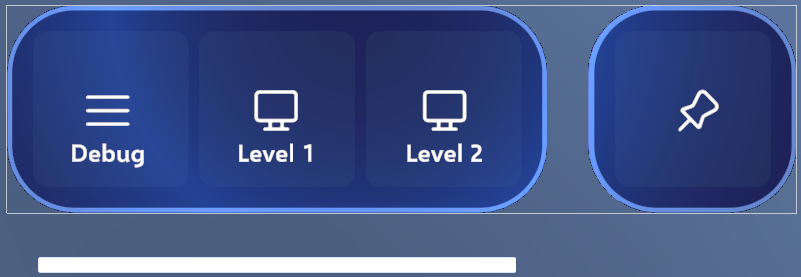
\includegraphics[width=0.8\textwidth]{images/menubar.png}
    \caption{Die Menüleiste besteht aus drei Buttons, einem Pin-Button und einer Grab-Bar.}
    \label{fig:menübar}
\end{figure}

\subsection{Beschreiben der Buttons}
Die Funktionalitäten der Buttons sind wie folgt:

\begin{itemize}
    \item \textbf{Debug-Button}\\
    Der Debug-Button ist ausschließlich für Entwickler vorgesehen. Beim Aktivieren öffnet sich ein erweitertes
    Menü oberhalb des Hauptmenüs, das zusätzliche Funktionen für das Bugfixing während des Betriebs bereitstellt.
    Vorhandene Optionen umfassen einen Reset-Button für Level 2, der bei Problemen mit der Platzierung von
    Inventarobjekten verwendet werden kann.

    \item \textbf{Pin-Button}\\
    Der Pin-Button ermöglicht das Fixieren des Menüs an einer geeigneten Stelle. Dies ist besonders nützlich,
    wenn der Benutzer sich an einen Tisch setzt und das Menü entsprechend positionieren möchte. Die
    Positionierung erfolgt mithilfe der Grab-Bar.

    \item \textbf{Grab-Bar}\\
    Die weiße Leiste (Grab-Bar) kann festgehalten werden, um das Menü frei zu bewegen. In Kombination mit dem
    Pin-Button ist eine präzisere Platzierung möglich.
\end{itemize}

\subsection{Laden der Level}
Das Betätigen eines dieser Buttons (Level 1, Level 2) löst das Skript SceneChanger aus. Dieser Code wechselt die geladene
Szene entsprechend. Die zu ladende Szene wird durch die Variable "sceneToLoad" definiert, die in Unity
festgelegt wird und das gewünschte Level angibt.


\begin{lstlisting}[language=C#, style=csharpstyle, caption=Auf Knopfdruck Szene wechseln.]
using UnityEngine;
using UnityEngine.SceneManagement;
public class SceneChanger : MonoBehaviour
{
public string sceneToLoad;

// Assign this method to the button's onClick event in the Unity Editor.
public void ChangeScene()
{
SceneManager.LoadScene(sceneToLoad);
Debug.Log("Button clicked. Loading scene: " + sceneToLoad);
}
}
\end{lstlisting}

\subsection{UI/UX}
\textbf{Blickzentrierung und Interaktionsmodelle}\\
Die Menüleiste bewegt sich auf Hüfthöhe mit dem Benutzer mit und ermöglicht so eine natürliche und intuitive Interaktion.
Der Benutzer kann die Bedienelemente einfach durch Blickkontakt auswählen, was die Benutzerfreundlichkeit erhöht und die
Bedienung der Anwendung erleichtert.\\
\\
\textbf{Konsistenz im Design}\\
Die klare Gestaltung der Buttons mit aussagekräftigen Symbolen trägt zur Konsistenz und Benutzerfreundlichkeit bei.
Eine einheitliche visuelle Sprache erleichtert es dem Benutzer, die Funktionen der Buttons zu verstehen, selbst wenn er
sie zum ersten Mal verwendet.\\
\\
\textbf{Kontextsensitive Funktionen}\\
Der Debug-Button bietet erweiterte Funktionen, die speziell für Entwickler relevant sind. Diese kontextsensitiven
Optionen sind wichtig für die Fehlersuche und tragen dazu bei, die Entwicklungszeit zu optimieren. Gleichzeitig bleibt
die Benutzeroberfläche für den Endbenutzer sauber und übersichtlich.\\
\\
\textbf{Anpassungsmöglichkeiten für den Benutzer}\\
Die Option, das Menü mit dem Pin-Button zu fixieren und mit der Grab-Bar frei zu bewegen, gibt dem Benutzer die
Kontrolle über die Positionierung des Menüs. Diese Anpassungsmöglichkeiten tragen dazu bei, die Anwendung an
verschiedene Nutzerszenarien anzupassen und die individuellen Bedürfnisse der Benutzer zu berücksichtigen.
Feedback und Animationen

\section{Ping Level}
In diesem Level wird das IT-Grundprinzip eines Pings zwischen zweier
PCs dargestellt. Das Kabel zwischen den zwei PCs wird von der
HoloLens getracked und mittels Kurvenberechnung wird dann eine
unsichtbare Kurve über dieses Kabel gezeichnet. Wenn dann der Benutzer
auf die Enter Taste auf einem PC drückt wird ein Ping-Paket simuliert
und auf dieser Kurve von einem PC zu dem anderen geschickt.

\subsection{Object Tracking}
Durch verwendung von bereitgestellten Technologien der HoloLens2
werden die zwei PCs und das Kabel getracked.
%Hier dann noch code zum Object Tracking einfügen

\subsection{Kurvenberechnung}
Durch Berechnung der Kurve wird das Kabel als Kurve gespeichert
und dadurch wird es ermöglicht, dass das 3D-Ping-Paket über diese
Kurve von einem PC zum anderen läuft.
%Hier dann noch code zur Kurvenberechnung einfügen

\section{Knappsack Problem Level}
In diesem Level wird das IT-Grundprinzip des Knappsack-Problems dargestellt.
Auf einem Tisch wird mittels Spatial Mapping die Oberfläche des Tisches
getracked und dann ein Spatial Anchor platziert. Auf diesem Anchor wird
anschließend der Inventar-Actor platziert. Außerdem liegen auf dem Tisch
verteilt reale Gegenstände die mit einem QR-Code versehen sind. Nimmt der
Spieler einen Gegenstand in die Hand, wird der QR-Code von der HoloLens2
erfasst. Darauf folgend wird der Inhalt des QR-Codes geladen und in einem
Fenster angezeigt. Der Benutzer kann die Gegenstände frei in das Inventar
verteilen und pro neuen Gegenstand wird ein Inventar-Value berechnet.
Wenn der Benutzer mit seiner Lösung zufrieden ist, kann er anschließend
durch einen Kopfdruck die perfekte Lösung in einem zweiten Inventar anzeigen
lassen.

\subsection{Spatial Anchors}
Spatial Anchors\footnote{Unity \cite{Anchor}} sind virtuelle Ankerpunkte in einer Augmented Reality (AR)- oder Mixed Reality-Umgebung, die dazu dienen,
virtuelle Objekte stabil und präzise in der realen Welt zu verankern. Diese Ankerpunkte ermöglichen es AR- und
MR-Anwendungen, die räumliche Beziehung zwischen virtuellen Objekten und der physischen Umgebung zu speichern und
beizubehalten. Spatial Anchors sind besonders wichtig, wenn es darum geht, AR-Objekte konsistent in der realen Welt
zu positionieren, unabhängig davon, wie sich der Benutzer oder das AR-Gerät bewegt.

\subsection{Managers}
In diesem Level werden mehrere von Unity und dem Mixed Reality Toolkit 3 bereits
bereitgestellten Manager \footnote{Medium \cite{Managers}} verwendet. Unter einer Manager
versteht man eine Komponente die einer Unity-Scene hinzugefügt wird die dazu dient,
bestimmte Aspekte oder Funktionen der Anwendung zu verwalten und zu stuern. Diese Manager
spielen eine wichtige Rolle in der Organisation und Kontroller verschiedener Teile der Unity-Anwendung.
In dem "Knappsack Problem Level" werden folgende Manager verwendet:
\begin{itemize}
    \item ARPlaneManager\footnote{Unity \cite{PlaneManager}}:\\
    Dieser Manager wird verwendet um in der Umgebung des Benutzers alle Horizontalen Flächen zu erkennen und zu tracken.
    Außerdem erleichtert er das platzieren von Objekten in der echten Welt.
    Diese Flächen werden anschließend mit einer Textur markiert. Wenn der User für die vorgeschriebene
    Zeit auf eine dieser Flächen schaut wird in der Mitte dieser Fläche das Inventar als 3D Objekt dargestellt. An dieses
    3D Objekt wird anschließend auch ein Spatial Anchor angehängt und in dem ARAnchorManager verwaltet.

    \item ARAnchorManager\footnote{Unity \cite{AnchorManager}}: \\
    Dieser Manager wird verwendet um AR-Anker in der AR-Welt und der echten Welt zu erstellen, zu verankern und zu verwalten.
    In dem "Knappsack Problem Level" wird dieser Manager gebraucht, weil wir das Inventar sowohl in der AR, als auch in
    der echten Welt verankern müssen. An der Stelle wo das Inventar verankert wird, wird anschließend ein ARAnchor \footnote{Unity \cite{Anchor}}
    erstellt, der von der HoloLens2 getracked wird.

    \item ARRaycastManager\footnote{Unity \cite{RaycastManager}}; \\
    Dieser Manager wird verwendet um aus einem Origin Punkt also in diesem Fall die Kamera der HoloLens2, raycasting durchzuführen.
    Diese Raycasts treffen dann auf bereits markierte und getrackte Planes. Wenn dies der Fall ist, ist bekannt, dass der
    Benutzer auf dieses Plane sieht. Dies ermöglicht dann eine akkurate Platzierung eines 3D Objekts in der realen Welt. \\

\end{itemize}
In dem folgendem Code Abscnhitt wird dargestellt wie die drei Manager alle zusammenspielen, um in der realen Welt
ein 3D Objekt zu verankern:

\begin{lstlisting}[language=C#, style=csharpstyle, caption=3D Objekt in der echten Welt platzieren]
using System.Collections.Generic;
using Unity.VisualScripting;
using UnityEngine;
using UnityEngine.XR.ARFoundation;
using UnityEngine.XR.ARSubsystems;

public class PlaceObjectOnLookedAtDesk : MonoBehaviour
{
    public ARRaycastManager raycastManager;
    public ARPlaneManager planeManager;
    public ARAnchorManager anchorManager;
    public GameObject objectToPlace;
    public float requiredLookTime = 3.0f;

    private ARPlane selectedDeskPlane;
    private float lookStartTime = -1f;
    private bool objectPlaced = false;
    private float heightOffset = 0.05f;

    //Gets called every frame
    void Update()
    {
        if (!objectPlaced)
        {
            List<ARRaycastHit> hits = new List<ARRaycastHit>();
            //if true the player is looking at a plane
            if (raycastManager.Raycast(new Vector2(Screen.width / 2, Screen.height / 2), hits, TrackableType.Planes))
            {
                ARPlane plane = planeManager.GetPlane(hits[0].trackableId);
                if (plane != null)
                {
                    if (selectedDeskPlane == null)
                    {
                        selectedDeskPlane = plane;
                        lookStartTime = Time.time; // Start the timer when a new plane is selected.
                        Debug.Log("Plane selected. Timer started.");
                    }
                    if (selectedDeskPlane == plane)
                    {
                        //start timer
                        float timeLookedAtPlane = Time.time - lookStartTime;
                        if (timeLookedAtPlane >= requiredLookTime)
                        {
                            PlaceObjectOnDesk(selectedDeskPlane);
                            objectPlaced = true;
                        }
                    }
                    else
                    {
                        selectedDeskPlane = null;
                    }
                }
                else
                {
                    selectedDeskPlane = null;
                }
            }
            else
            {
                selectedDeskPlane = null;
            }
        }
    }

    void PlaceObjectOnDesk(ARPlane deskPlane)
    {
        // Disable the plane manager to stop further plane detection.
        planeManager.enabled = false;
        // Disable this script so it won't run again.
        gameObject.SetActive(false);
        // Calculate the object's position above the center of the plane.
        Vector3 objectPosition = deskPlane.center + Vector3.up * heightOffset;
        // Instantiate the object and place it at the calculated position.
        Instantiate(objectToPlace, objectPosition, Quaternion.identity);


        /*
        //This code handles the calculation for the placement position and also attaches an ARAnchor to the placed Object
        // Disable the plane manager to stop further plane detection.
        planeManager.enabled = false;

        // Disable this script so it won't run again.
        gameObject.SetActive(false);

        // Calculate the object's position above the center of the plane.
        Vector3 objectPosition = deskPlane.center + Vector3.up * heightOffset;

        //Create Anchor
        ARAnchor newAnchor = anchorManager.AddComponent<ARAnchor>();
        GameObject anchorVisual = Instantiate(objectToPlace, objectPosition, Quaternion.identity);
        anchorVisual.transform.parent = newAnchor.transform;
        */
    }
}

\end{lstlisting}

\subsection{QR-Code Tagging}
Generierte QR-Codes werden auf die realen Objekte geklebt. In diesen QR-Codes werden
wichtige Informationen zu den Objekten gespeichert. Darunten sind folgende Elemente:
Gewicht, Wert und eine kurze Beschreibung zu diesem Objekt.

\subsection{QR-Code Tracking}
Durch Verwendung der integrierten Kamera rendert die HoloLens2 existente QR-Codes an
der Originalen Positionen in 3D-Objekte. Mittels tracking kann dann auch der Inhalt
der getracked QR-Codes geladen werden.
%Genauer Beschreibung + wenn vorhanden Code und Blueprints von QR-Code-Tracking hinzufügen

\subsection{Knappsack-Algorithmus}
%Hier kommt dann ein Bild von dem Level Blueprint + Custom Code vom Knappsack Algorithmus mit erklärung
Durch Interaktion zwischen echten und 3D-Obejekt können

\subsection{Unit-Tests}
Durch Hilfe von Unit-Tests wird versichert, dass der implementierte Knappsack-Algorithmus
richtig und performant funktioniert.
%Genauere Erklärung + Custom Code der UnitTests

\section{Performance}
Performance-Messung
